\documentclass{standalone}

\usepackage{tikz,amsmath}
\usetikzlibrary{calc,snakes,decorations}

\begin{document}
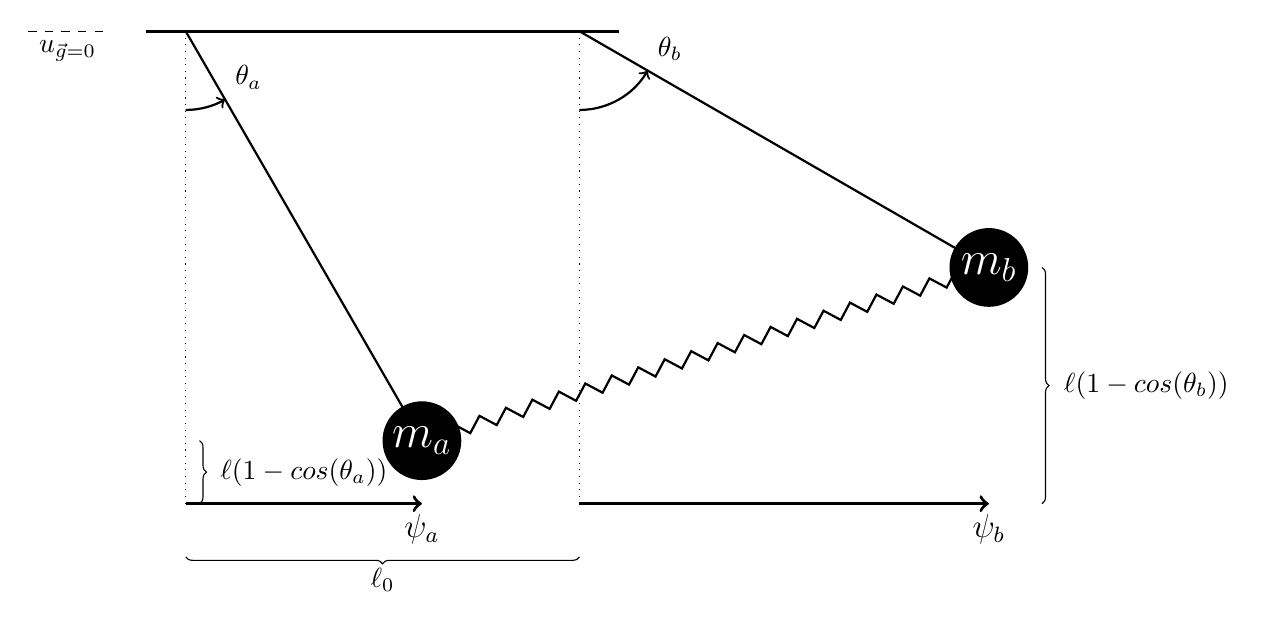
\begin{tikzpicture}

\draw[very thick](-3,6)--(3,6);

\coordinate (A) at (0.5,0.8);
\coordinate (B) at (7.7,3);

\draw[dashed](-4.5,6)--node[anchor=north]{$u_{\vec{g}=0}$}(-3.5,6);

\draw[dotted,thin](-2.5,0)--(-2.5,6);
\draw[dotted,thin](2.5,0)--(2.5,6);

\draw[thick,->](-2.5,5)arc(-90:-60:1)node[anchor=south west]{$\theta_a$};
\draw[thick, ->](2.5,5) arc(-90:-30:1)node[anchor=south west]{$\theta_b$};

\draw [decoration={brace,raise=5pt}, decorate] (-2.5,0|-A) --(-2.5,0);
\node at (-1,0.4)[]{$\ell(1-cos(\theta_a))$};

\draw [decoration={brace,raise=5pt,mirror},decorate] (8.2,0)--(8.2,0|-B);
\node at (9.7,1.5)[]{$\ell(1-cos(\theta_b))$};

\draw[decoration={brace,raise=5pt,mirror},decorate](-2.5,-0.5)--(2.5,-0.5);
\node at (0,-0.7) [anchor=north] {$\ell_{0}$};

\draw[thick](-2.5,6)--(A);
\draw[thick](2.5,6) --(B);
\draw[thick,snake=zigzag](A)--(B);

\fill (A) node {\color{white} \LARGE{$m_a$}} circle(0.5);
\fill (B) node {\color{white} \LARGE{$m_b$}} circle(0.5);

\draw[very thick, ->](-2.5,0)--(A|-0,0)node[anchor=north]{\large {$\psi_a$}};
\draw[very thick, ->](2.5,0)--(B|-0,0)node[anchor=north]{\large {$\psi_b$}};

\end{tikzpicture}
\end{document}